\chapter{Visão Geral}

Para embasar e planejar o projeto a ser desenvolvido, uma proposta de
arquitetura precisa ser feito. Neste capítulo será apresentado a proposta do projeto UMISS,
sendo explanado as arquiteturas de cada subsistema.

\section{Subsistema - Processamento de Sinais e Monitoramento}

O subsistema de controle e monitoramento terá como grande objetivo a aquisição
dos sinais do paciente, a disponibilização desses recursos para os
interessados, e a notificação dos responsáveis em casos de eventos críticos.
Sua arquitetura pode ser dividido em três grandes
módulos: o módulo que chamaremos \textbf{módulo eletrônico}, que conterá
grande parte dos componentes eletrônicos do projeto,
o \textbf{módulo servidor remoto}, que será um servidor remoto disponível
para ser consumido por outros serviços, e o \textbf{módulo aplicativo},
que será uma solução em aplicativo para ser utilizado pelos interessados.

\subsection{Módulo Eletrônico}
O módulo eletrônico será composto principalmente por sensores, amplificadores,
filtros, conversores, e um sistema embarcado.

Os sensores terão como principal papel a extração dos sinais vitais do
paciente, e serão acoplados a estrutura da cadeira, de forma que algum
membro do paciente fique em contato com o sensor, permitindo assim a
aquisição do sinal.

Os amplificadores e filtros serão responsáveis pelo condicionamento do sinal. 
Os sinais adquiridos serão amplificados, por tratarem-se de sinais de baixa 
amplitude, e filtrados para atenuação de ruídos de frequências indesejadas.

Os conversores DAC (\textit{Digital Analog Converter}) terão como papel a conversão 
dos sinais analógicos adquiridos do usuário para formato digital, para que
possam ser processados pelo processador central do sistema.

Um sistema embarcado será responsável por receber os sinais do paciente,
processá-los e utilizá-los em tarefas específicas, e, por fim, despachar os
dados para o módulo servidor remoto.

\subsection{Módulo Servidor Remoto}
O módulo servidor remoto é dividido nos seguintes componentes: um servidor remoto
e gerência de configuração do servidor.

O servidor remoto será um servidor hospedado fora da rede-interna da parte
eletrônica, e poderá ser acessado via \textit{internet}. Se comunicará com
o sistema embarcado da parte eletrônica utilizando comunicação
\textit{via socket}\footnote{\url{https://docs.oracle.com/javase/tutorial/networking/sockets/definition.html}},
apresentará dados para o aplicativo, e o notificará da ocorrência de eventos
críticos.

A gerência de configuração do servidor será composta principalmente de
configurações e \textit{scripts} que vão permitir a manutenção e
interoperabilidade entre o servidor e outros recursos.

\subsection{Módulo aplicativo}

O aplicativo só tem si próprio como componente, e será utilizado regularmente
pelos responsáveis do paciente; estará preparado para receber as notificações
do servidor e para mostrar os dados em tempo real.

\subsection{Integração entre os módulos}

\begin{figure}[H]
  \centering
    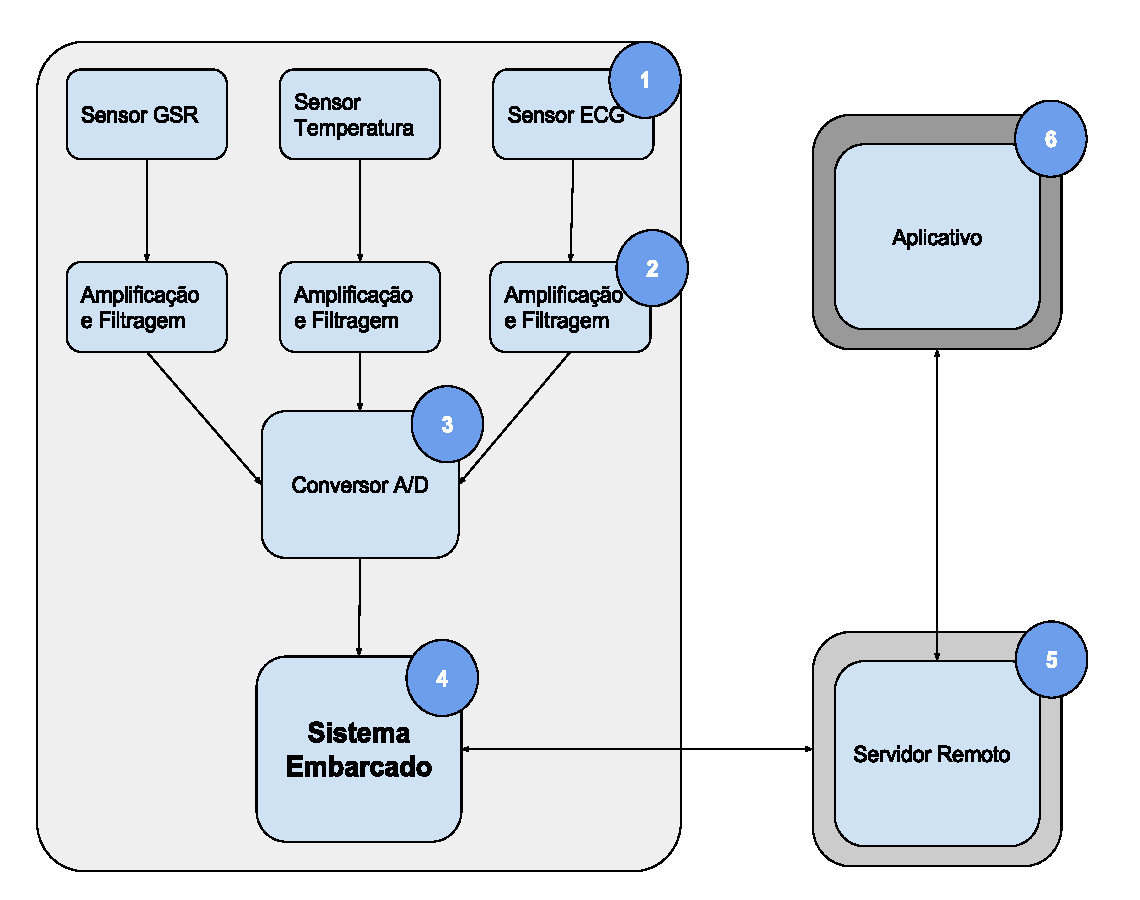
\includegraphics[width=\textwidth]{figuras/arquitetura-monitoramentoecontrole.eps}
  \caption{Fluxo típico do subsistema de Monitoramento e Controle}
  \label{fig:arquitetura-monitoramento-e-controle}
\end{figure}

O passo (1) do subsistema é atuado pelos sensores, que extraírão sinais do paciente;
o passo (2) será atuado pelos amplificadores e filtros, e tratarão o sinal
extraído pelos sensores no passo anterior; no passo (3) os sinais tratados
são convertidos para formato digital, para que possam ser lidos pelo sistema
embarcado; no passo (4) o sistema embarcado recebe as informações do conversor
e abre conexão com o servidor remoto - após, envia as informações recebidas,
quando necessário; no passo (5) o servidor remoto recebe dados do sistema
embarcado e passa informações importantes para o aplicativo, e, por fim,
no passo (6), o aplicativo recebe as informações.

\subsection{Tecnologias Utilizadas}

\subsubsection{Servidor Django}
\label{sub:servidor_django}
O passo (5), retratado na Figura \ref{fig:arquitetura-monitoramento-e-controle},
representa o servidor remoto, que irá receber as informações de todas as
estações embarcadas do sistema. Este será responsável por receber, processar
e se comunicar com os dispositivos móveis cadastrados no sistema. Para tal,
será utilizado uma linguagem de programação compatível com a que será utilizada
no software embarcado, que será escrito em python. Desta maneira, todo
o servidor proverá serviços utilizando python.

Um Framework robusto e já bastante consolidado na comunidade python é o Django.
Este é bem completo e possui várias ferramentas que auxiliam no desenvolvimento.
O django possui um framework para API's Rest, que será o padrão utilizado pelos
clientes para se comunicarem, chamado de DjangoRestFramework. Este é muito poderoso
e de alta produtividade.

Estas três ferramentas irão compor juntas o passo (5).

\subsubsection{Sistema Embarcado}
Um sistema central de processamento foi selecionado para compor o passo (4).
A placa de desenvolvimento Raspberry Pi 3 Model B, apresentada na Figura \ref{rasp} foi selecionada para
a execução do processamento dos dados adiquiridos por possuir, além de alta 
velocidade de processamento, conexão WiFi, o que possibilita a comunicação 
com o servidor remoto, de acordo com os requisitos do projeto.

\begin{figure}[H]
  \centering
    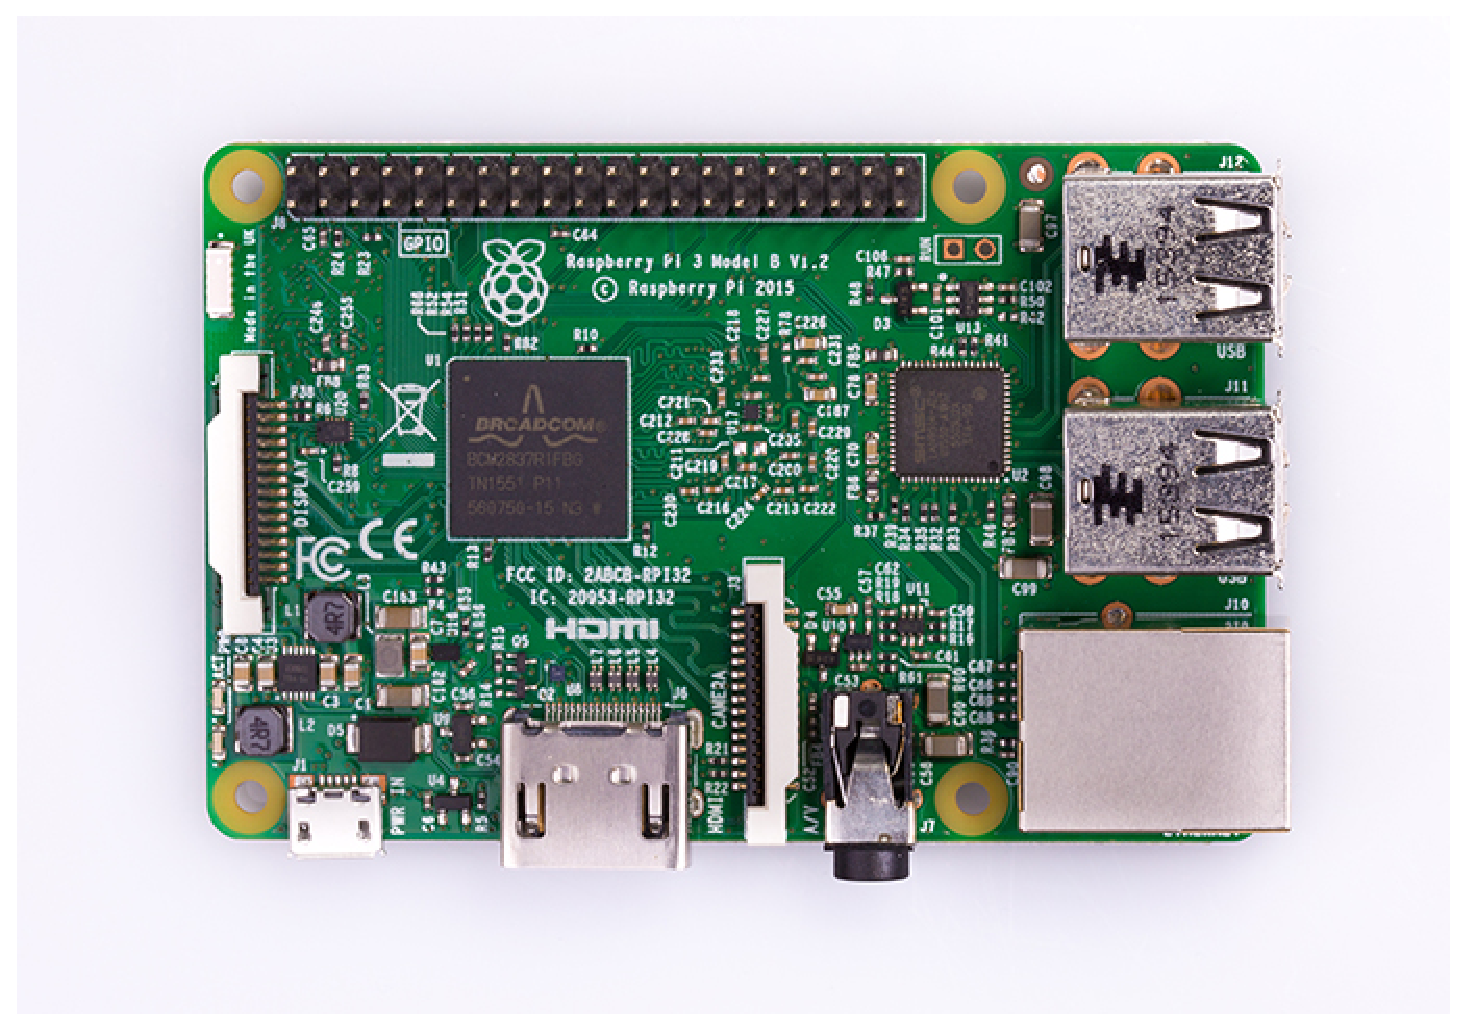
\includegraphics[keepaspectratio=true,scale=0.6]{figuras/rasp.eps}
  \caption{Microcomputador Raspberry Pi 3 Modelo B.}
  \label{fig:rasp}
\end{figure}

\subsubsection{Conversor AD}
Para a conversão dos sinais analógicos para digitais, foi selecionado o conversor 
AD ADS1115, apresentado na Figura \ref{ads}, que possui quatro canais de entrada analógica, resolução de 16 bits 
e amostragem de 800Hz. 

\begin{figure}[H]
  \centering
    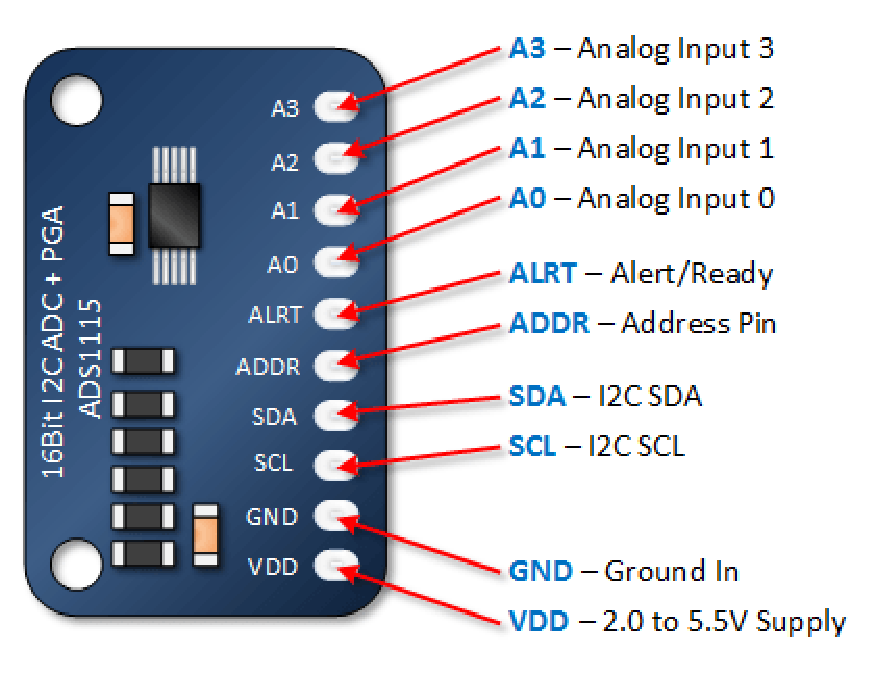
\includegraphics[keepaspectratio=true,scale=0.7]{figuras/ads.eps}
  \caption{Conversor analógico-digital ADS1115.}
  \label{fig:ads}
\end{figure}

Preocupações de importante ressalte durante a seleção do 
conversor 
foram sua resolução e amostragem. O conversor ADS1115 possui alta 
resolução com 
seus 16 bits, possibilitando uma captura mais refinada dos sinais 
de pequena 
variação. Além disso, possui amostragem de 800Hz, necessária 
para captura 
de sinais de eletrocardiograma (ECG) e frequência cardíaca, 
que possuem 
frequências úteis até 300Hz, dessa forma, 800Hz de amostragem 
mostra-se 
suficente para boa captura desses sinais, entre os outros necessários para o projeto.

\subsubsection{Amplificadores de Intrumentação e Operacionais}
Para os sistemas de amplificação dos sinais capturados e condicionamento dos mesmos, serão utilizados amplificadores operacionais e de intrumentação.

A amplificação e captura de sinais vitais de baixa amplitude de forma ótima é 
uma tarefa que requer um amplificador de instrumentação, com ganho regulável 
por divisores de tensão, permitem aplicação de alto ganho sem aplicar novos 
ruídos ao sinal. Para a amplificação dos sinais para frequência cardíaca 
serão utilizados amplificadores INA118 e INA128, fabricados pela \textit{Texas Instruments}. Além, para a filtragem dos sinais, serão implemetadas 
topologias de filtragem analógica do tipo \textit{Sallen-Key}, que necessitam da 
utilização de amplificadores operacionais para seleção das frequências 
de corte desejadas, para estes, serão utilizados amplificadores TL084, 
da \textit{Texas Instruments}, por maior concentração de amplificadores 
por chip e pelo baixo ruído apresentado por estes amplificadores.

\subsubsection{Aquisição de Sinais}
Para a aquisição dos sinais do usuário, serão utilizados sensores e eletrodos específicos para cada tipo de sinal. Para a captura dos sinais de resistência galvânica da pele (GSR), pela qual é possível identificar alterações de estresse do usuário e prováveis convulsões ou crises hipoglicêmicas, serão utilizados eletrodos com contatos de prata ou alumínio, em contato com os dedos ou pulso do usuário.

Para a aquisição dos sinais de temperatura corporal, serão utilizados termistores, que consistem em resistores que apresentam variação de resistência para variações de temperaturas, regidas pela equação de \textit{Steinhart-Hart} \cite{gregg}, para esses termistores, haverão, no sistema embarcado, rotinas para definir a temperatura corporal a partir de valores de tensão recebidos.

Além, para captura de sinais de frequência cardíaca, serão utilizados sensores ópticos ou eletrodos de contato para captura dos sinais de eletrocardiograma (ECG).

Na Figura \ref{sensors} é possível visualizar modelos comuns dos sensores e eletrodos utilizados.

\begin{figure}[H]
  \centering
    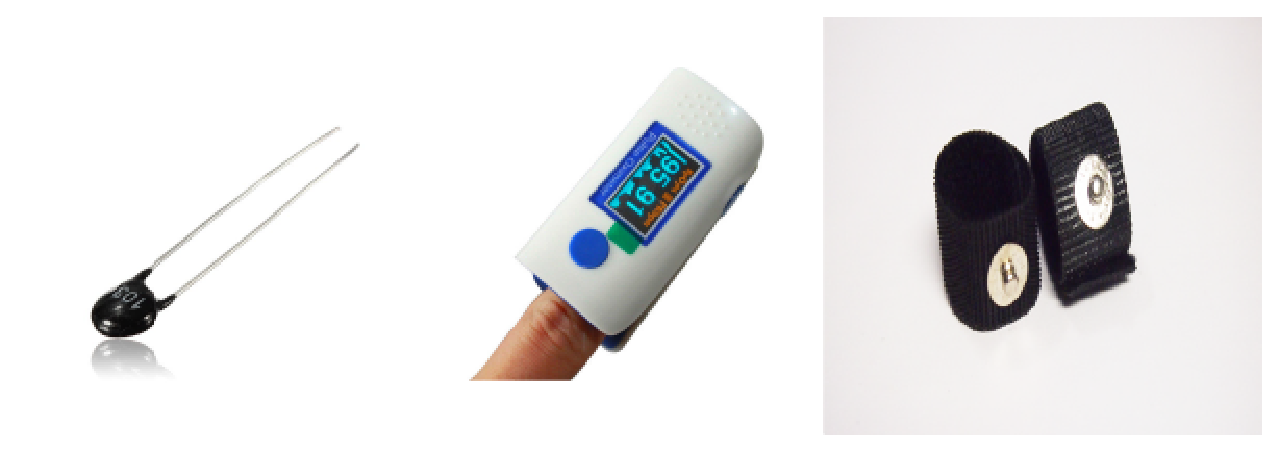
\includegraphics[width=\textwidth]{figuras/sensors.eps}
  \caption{Sensores e eletrodos para captura de sinais: Termistor NTC 10K para temperatura, oximetro de dedo para frequência cardíaca e contatos de prata para captura de GSR.}
  \label{fig:sensors}
\end{figure}

\section{Subsistema - Controle e Alimentação}
Neste projeto serão usados motores de corrente contínua a fim de movimentar o conjunto
cadeira $+$ paciente, esses motores devem ser capazes de fornecer o torque solicitado
nas diversas situações, como o uso com carga elevada e a movimentação em aclives.
Serão usados circuitos driver para o controle de tais motores. De forma simplificada
uma máquina de corrente contínua é formada por duas partes distintas, a parte
estacionária chamada de estator, onde estão localizados os polos indutores e o
enrolamento de campo, e a parte girante chamada de rotor onde se encontram as
bobinas do enrolamento de armadura, bem como o comutador  \cite{bim}. O comutador
é um conjunto de barras isoladas entre si e conectadas no eixo do rotor, ele tem
a função de mudar o sentido da corrente que passa pelo enrolamento de armadura.
Um exemplo de rotor e estator é mostrado na figura~\ref{fig:rotor}.

\begin{figure}[H]
  \centering
    \includegraphics[width=\textwidth]{figuras/rotor.eps}
  \caption{Exemplo de um estator e um rotor \cite{bim}}
  \label{fig:rotor}
\end{figure}

\subsection{Dimensionamento do Sistema Eletromecânico}

Para a análise das características requeridas de torque e potência foram estimados
massa do sistema foi estimada como $150 kg$, a sua velocidade máxima como $3 km/h$
e o tempo para atingir tal velocidade como $4$ segundos. A partir desses dados é
possível calcular a força necessária para colocar a cadeira em movimento bem como
para a acelerar até a velocidade máxima. Dividindo a velocidade pelo tempo necessário
para se alcançar a velocidade é possível calcular a aceleração.

\begin{equation}
a = \frac{V}{t} = \frac{3}{3,6\cdot 4} = 0,20834  \frac{m}{s^2}
\end{equation}

Em seguida calculamos a força necessária para acelerar a massa de $150 kg$.

\begin{equation}
F_{a} = M \cdot a = 150 \cdot 0,20834 = 31,25 N
\end{equation}

Também deve ser levado em conta a força necessária para colocar a massa da cadeira
em movimento, e usamos um valor de coeficiente de atrito estático $a = 0,3$.

\begin{equation}
F_{r} = M \cdot g \cdot a = 441,45 N
\end{equation}

Então, a força total solicitada é dada pela soma da força de resistência ao movimento
e da força de aceleração.

\begin{equation}
F_{T} = F_{a} + F_{r} = 472,7 N
\end{equation}

Finalmente é possível calcular o torque solicitado utilizando o raio do eixo do
motor de $4mm$.

\begin{equation}
T = F_{T} \cdot R = 472,7 \cdot 0,004 = 1,8908 N\cdot m
\end{equation}

A potência requerida é calculada multiplicando-se o torque pela velocidade máxima.

\begin{equation}
P = T \cdot V = 441,45 \cdot 0,83334 = 367 W
\end{equation}

\subsection{Especificações do Motor}

Serão utilizados dois motores Bosch modelo GPB F006 KM0 611, que tem aplicações
em sistemas de arrefecimento, o emprego dos dois motores satisfaz as exigências
de potência e torque do sistema. As curvas características desse motor e seus
dados técnicos são mostrados a seguir.

\begin{figure}[H]
  \centering
    \includegraphics[width=\textwidth]{figuras/motor.eps}
  \caption{Curvas de motor GPB F006 KM0 611 (Bosch)}
  \label{fig:motor}
\end{figure}

\begin{table}[h]
\centering
\vspace{0.5cm}
\begin{tabular}{|l|l|}
\hline
Item                & Especificação \\
\hline
Tensão Nominal      & 12 V \\
Potência Nominal    & 305 W \\
Rotação Nominal     & 2600 rpm \\
Corrente Nominal    & 25A \\
Torque Nominal      & 350 Ncm \\
Peso                & 1,585 kg \\
\hline
\end{tabular}
\caption{Dados motor GPB F006 KM0 611 (Bosch)}
\label{tab:dadosmotor}
\end{table}

\subsection{Dimensionamento da Bateria}

Sabe-se que a potência necessária para movimentar a cadeira de rodas é de $367 W$,
também sabe-se que a tensão nominal do motor GPB F006 KM0 611 da Bosch é de $12V$,
logo as baterias devem ser capazes de fornecer essa potência para o sistema por
pelo menos 3 horas. Para determinar qual bateria usar deve ser estimada a
capacidade em Ah, também devem as suas dimensões e peso, outro fator importante
é o custo, já que o projeto tem orçamento limitado \cite{costa}.

A bateria a ser utilizada deve ter uma tensão de $12V$, pois esse valor é
compatível tanto com a necessidade dos motores quanto com a disponibilidade dos
modelos de mercado. Tendo em vista a potência calculada e a tensão estabelecida
é possível calcular a corrente necessária.

\begin{equation}
P = V \cdot I
\end{equation}

\begin{equation}
I = \frac{367}{12} = 30,58 A
\end{equation}

Com esse valor de corrente e o tempo de trabalho do sistema é possível calcular
a carga da bateria.

\begin{equation}
C = I \cdot t = 30,58 \cdot 3 = 91,74 Ah
\end{equation}

Sabe-se que a bateria não deve ser totalmente descarregada, pois isso diminui a
vida útil da mesma, logo deve ser utilizado um fator de profundidade de descarga,
que nesse caso será de $80\%$ \cite{KARASINSKI}.

\begin{equation}
C = \frac{91,74}{0,8} = 114,675 Ah
\end{equation}

Um ponto importante no dimensionamento é o fato de o sistema de movimentação não
operar em plena carga a todo tempo, havendo momentos em que a potência necessária
é reduzida ou até mesmo nula, situação onde a cadeira está parada, portanto deve
se estimar um fator de demanda para os motores, para esse projeto o valor
adotado de para o fato de demanda será de $0,75$. Com isso temos que a carga
necessária será de:

\begin{equation}
C = 114,675 \cdot 0,75 = 86Ah
\end{equation}

Uma possível solução que prioriza a variável custo é a utilização de $3$ baterias
de chumbo-ácido de $30 Ah$ ligadas em paralelo.

\section{Subsistema - Projeto Estrutural}

\section{Outros}

\subsection{Integração Contínua}
